\documentclass[journal, a4paper, 12pt]{IEEEtran}

\usepackage{graphicx} 

\usepackage{url}     

\usepackage{amsmath}  

\usepackage{listings}
\usepackage{xcolor}

\usepackage{epstopdf}
\lstset{ %
  backgroundcolor=\color{white},   % choose the background color; you must add \usepackage{color} or \usepackage{xcolor}
  basicstyle=\footnotesize,        % the size of the fonts that are used for the code
  breakatwhitespace=false,         % sets if automatic breaks should only happen at whitespace
  breaklines=false,                 % sets automatic line breaking
  captionpos=b,                    % sets the caption-position to bottom
  deletekeywords={...},            % if you want to delete keywords from the given language
  escapeinside={\%*}{*)},          % if you want to add LaTeX within your code
  extendedchars=true,              % lets you use non-ASCII characters; for 8-bits encodings only, does not work with UTF-8
  frame=l,	                   % adds a frame around the code
  keepspaces=true,                 % keeps spaces in text, useful for keeping indentation of code (possibly needs columns=flexible)
  keywordstyle=\color{blue},       % keyword style
  language=Python,                 % the language of the code
  otherkeywords={*,...},           % if you want to add more keywords to the set
  %numbers=left,                    % where to put the line-numbers; possible values are (none, left, right)
  %numbersep=5pt,                   % how far the line-numbers are from the code
  showspaces=false,                % show spaces everywhere adding particular underscores; it overrides 'showstringspaces'
  showstringspaces=false,          % underline spaces within strings only
  showtabs=false,                  % show tabs within strings adding particular underscores
  stepnumber=2,                    % the step between two line-numbers. If it's 1, each line will be numbered
  tabsize=2,	                   % sets default tabsize to 2 spaces
  %title=\lstname                   % show the filename of files included with \lstinputlisting; also try caption instead of title
  xleftmargin=0.5cm,
  frame=tlbr,
  framesep=0pt,
  framerule=0pt
  }
% Your document starts here!
\begin{document}

% Define document title and author
	\title{Machine Problem 1 Report}
	\author{Yihui He*
	\thanks{*Exchange student, 2nd year CS undergrad from  Xi'an Jiaotong University, eli.he@foxmail.com}}
	\markboth{CS291K}{}
	\maketitle

% Write abstract here
% \begin{abstract}
% 	The short abstract (50-80 words) is intended to give the reader an overview of the work.
% \end{abstract}

% Each section begins with a \section{title} command
\section{Implementation}
% \PARstart{}{} creates a tall first letter for this first paragraph
	\PARstart{}{Key} points of implementing each part of neural network are illustrated as follow. \\
	All matrix multiplications are done via np.dot(). Element-wise matrix operation is done via "*".
\subsection{Forward pass and Loss}
	In Forward pass \textit{np.maximum} between z and 0, is used to represent \textit{ReLU} activation function.
	
	In Softmax, first raise \textit{scores} to the power of e element-wisely, then divide each element by row sum, finally we get $ a^{(3)} $.
	
	When computing Loss, pick up each true label element in each row is tricky: \textit{a3[range(len(a3)),y]}. Part of Forward pass is shown below. Other part of codes can be found in source files.
\begin{lstlisting}
a2=np.maximum(X.dot(W1)+b1,0)
scores=a2.dot(W2)+b2
a3=exp_scores\
  /(np.sum(exp_scores,1))[:,None]
\end{lstlisting}
\subsection{Backward pass and Gradient check}
	Firstly for each input, we need to compute $\delta_j^{(3)}$ for each output unit $j$:
	\[\delta_j^{(3)}=
	\begin{cases}
		\frac{1}{N}p(Y=j|X=x_i)-\frac{1}{N} &j=y_i\\ 
		 \frac{1}{N}p(Y=j|X=x_i) &j\neq y_i
	\end{cases}\]
\begin{lstlisting}
delta_3=a3
delta_3[range(len(a3)),y]=\
  a3[range(len(a3)),y]-1
delta_3/=len(a3)
grads['W2']=a2.T.dot(delta_3)+reg*W2
grads['b2']=np.sum(delta_3,0)
\end{lstlisting}
	Secondly, in the front hidden layer, for each input, we need to compute $\delta_j^{(3)}$ for each hidden node $j$:
	\[\delta_j^{(2)}= (w_j^{(2)})^T\delta^{(3)}\circ f'(z_j^{(2)})\]
	Note that, the second operator is Hadamard product.
\begin{lstlisting}
dF=np.ones(np.shape(a2))
dF[a2==0.0]=0
delta_2=delta_3.dot(W2.T)*dF
grads['W1']=X.T.dot(delta_2)+reg*W1
grads['b1']=np.sum(delta_2,0)
\end{lstlisting}
	To avoid divide by zero in gradient check, I made a small modification to the formula:
	\[\frac{\left|A-B\right|}{max(10^{-8},\left|A+B\right|)}\leq \delta\]
	max errors among inputs are as follow:\\
	$w_1$ 3.56e-09  $b_1$   2.74e-09\\
	$w_2$ 3.44e-09 $b_2$   4.45e-11
\subsection{Train and Predict}
	To perform a minibatching, \textit{np.random.choice} can be used, and set \textit{replace=True} to avoid same inputs being used. Then update each hyperparameter using SGD.
\begin{lstlisting}
rand_idx=np.random.choice(
  num_train,batch_size,replace=False)
X_batch=X[rand_idx]
y_batch=y[rand_idx]
for var in self.params:
  self.params[var]-=\
    learning_rate*grads[var]
\end{lstlisting}
As for predicting, run forward propagation, and use \textit{np.argmax( ,1)}to find predicted \textit{y} for each input.
\begin{lstlisting}
y_pred=np.argmax(np.maximum(0,\
  (X.dot(self.params["W1"])\
  +self.params['b1']))\
  .dot(self.params['W2'])+\
  self.params['b2'],1)
\end{lstlisting}
\section{Model Building}
	Basically there are two ways to tune a neural net: grid search and random search. For simplicity, I employ grid search to tune 3 hyperparameters: number of neurons in the hidden layer, regularization strength, and learning rate. My tuning procedure is twofold. First, run a coarse-grained search. Second, based on the result of first step, run a fine-grained search around top results.
	
	For coarse-grained search, Number of neurons range from 50 to 550, step 50. Regularization strength and learning rate are selected from geometrical sequences. Regularization strength range from $0.5\times10^{-3}$ to $0.5\times10^{2}$, with ratio $10$. Learning rate range from $1\times10^{-5}$ to $1\times10^{-1}$, with ratio $10$. 
	During this, top results have about \textbf{45\%} validation accuracy. Some Top results are shown below:

	
	% This is how you define a table: the [!hbt] means that LaTeX is forced (by the !) to place the table exactly here (by h), or if that doesnt work because of a pagebreak or so, it tries to place the table to the bottom of the page (by b) or the top (by t).
	\begin{table}[!hbt]
		\centering
		\caption{top accuracy}
		\label{top-accuracy}
		\begin{tabular}{|l|l|l|l|}
			\hline

			\multicolumn{1}{|p{1cm}|}{\centering hidden \\ neurons}
			
			&\multicolumn{1}{|p{1cm}|}{\centering learning \\ rate}
			&\multicolumn{1}{|p{2cm}|}{\centering regularization \\ strength}
			&\multicolumn{1}{|p{1.5cm}|}{\centering validation \\ accuracy}\\
			\hline
			350 & 0.001    & 0.05   & 0.516 \\
			\hline
			400 & 0.001    & 0.005  & 0.509 \\
						\hline
			250 & 0.001    & 0.0005 & 0.505 \\
						\hline
			250 & 0.001    & 0.05   & 0.501 \\
						\hline
			150 & 0.001    & 0.005  & 0.5   \\
						\hline
			500 & 0.001    & 0.05   & 0.5  \\
			\hline
	\end{tabular}
\end{table}
	For fine-grained search, I picked up one of the above top results. 
	And search around it's hyperparameters. It can reach a validation accuracy of \textbf{50\%}. 
	After found a suitable set of hyperparameters, I start tuning numbers of iterations, and batch size. 
	Finally, our original neural network reach a validation accuracy of \textbf{52\%}.
\section{Extra Credits}
I put results in the next section, in order to compare our original two-layers neural network, with other enhanced neural networks.
\subsection{momentum and other update methods}
	Implementation of momentum needs to change hyperparameters update code in \emph{train}.
\begin{lstlisting}
self.cache[param]=np.zeros(
grads[param].shape)
self.cache[param]=arg*self.cache[param
-learning_rate*grads[param]
self.params[param]+=self.cache[param]
\end{lstlisting}
	In order to tune momentum parameter and compare result with SGD, all other hyperparameters are fixed. Intuitively, momentum should speed up training procedure. I test momentum and SGD with 1000 iterations to see their converge rate.  It turns out that enjoys better converge rates.
	
	I also tried other update methods. 
	Nesterov momentum, which is a look-ahead version of momentum.
\begin{lstlisting}
v_prev = cache[param]
cache[param]=arg*cache[param]\
  -learning_rate*grads[param]
self.params[param]+=-arg*v_prev\
  +(1+arg)*cache[param]
\end{lstlisting}
RMSprop, which is a per-parameter adaptive learning rate method.
\begin{lstlisting}
cache[param]=arg*cache[param]\
+(1-arg)*np.power(grads[param],2)
self.params[param]-=learning_rate\
*grads[param]\
/np.sqrt(cache[param]+1e-8)
\end{lstlisting}
It turns out that, Momentum, Nesterov momentum and RMSprop all have a better converge rate than SGD. However, difference between these three update methods is ambiguous. Performances of these methods are compared in table~\ref{Differences between update methods}
\begin{table}[!hbt]
	\centering
	\caption{Differences between update methods}
	\label{Differences between update methods}
	\begin{tabular}{lllll}
		accuracy & Train & Validation & Test &  \\
		SGD      & .27   & .28        & .28  &  \\
		Momentum & .49   & .472       & .458 &  \\
		Nesterov & .471  & .452       & .461 &  \\
		RMSprop  & .477  & .458       & .475 & 
	\end{tabular}
\end{table}
				
\subsection{Dropout}
	Because we only have one layer of hidden nodes,
	dropout only needs to be performed once per batch. In code, it only needs minor change to Forward pass. 
\begin{lstlisting}
a2*=(np.random.randn(*a2.shape)<p)/p
\end{lstlisting}
	Dropout is said to be a easy way to prevent overfitting,
	and it is also an ensemble of multi models which should enhance performance.
	So I test it with more hidden neurons(500 hidden neurons).
	Dropout rate is set to be 30\% , 50\% and 70\% empirically.
	It turns out that the results from these three dropout rates do not differ a lot,
	with test accuracy ranging from \textbf{54\%} to \textbf{56\%}. And it also shows that,
	with out L2 regularization, dropout is able to constrain train accuracy not too higher than validation accuracy,
	which is 73\%.
	
	% This is how you include a eps figure in your document. LaTeX only accepts EPS or TIFF files.

	\begin{figure}[!hbt]
		% Center the figure.
		\begin{center}
			% Include the eps file, scale it such that it's width equals the column width. You can also put width=8cm for example...
			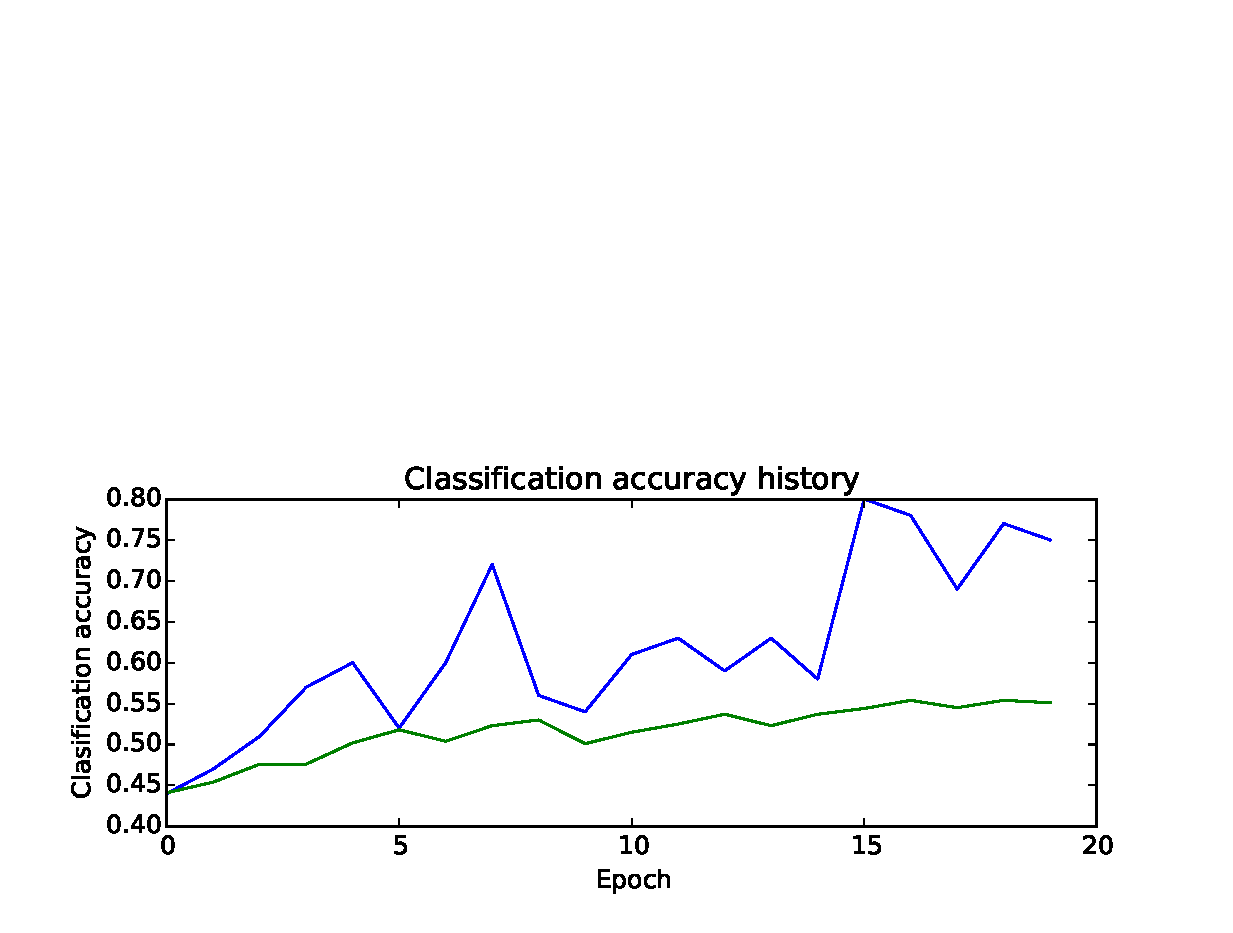
\includegraphics[width=\columnwidth]{dropout}
			% Create a subtitle for the figure.
			% Define the label of the figure. It's good to use 'fig:title', so you know that the label belongs to a figure.
			\label{fig:tf_plot}
		\end{center}
	\end{figure}
	
	
\subsection{Initialization method}
I tried 3 different ways of initialization:$\text{N}(0,1)\sqrt{1/n}$,
$\text{N}(0,1)\sqrt{2/(n_{in} + n _{out}})$,$\text{N}(0,1)\sqrt{2/n}$. Comparing with the our original initialization: $10^{-4}\text{N}(0,1)$, some outperform it. The neural network I'm testing on have 500 hidden neurons. I trained it 10000 iterations, 100 batch size, with dropout and momentum.

 In our case, we have 3072 input neurons, so $\text{N}(0,1)\sqrt{1/n}$ actually is $3.3\times10^{-4}$, whose weights are 3 times bigger than our original initialization. It is terrible at first 100 iterations. It reaches loss of 33.161757. 
 
 We only 10 output neurons. So $\text{N}(0,1)\sqrt{2/(n_{in} + n _{out}})$ and $\text{N}(0,1)\sqrt{2/n}$ do not differ so much between each other. Although, these two initialization methods' weights are 1.5 times bigger than our original initialization.Loss changing is almost the same as our original initialization. But maybe these methods are better, they are related to the input and output rather than a hand setting value.
 
 	\begin{figure}[!hbt]
 		% Center the figure.
 		\begin{center}
 			% Include the eps file, scale it such that it's width equals the column width. You can also put width=8cm for example...
 			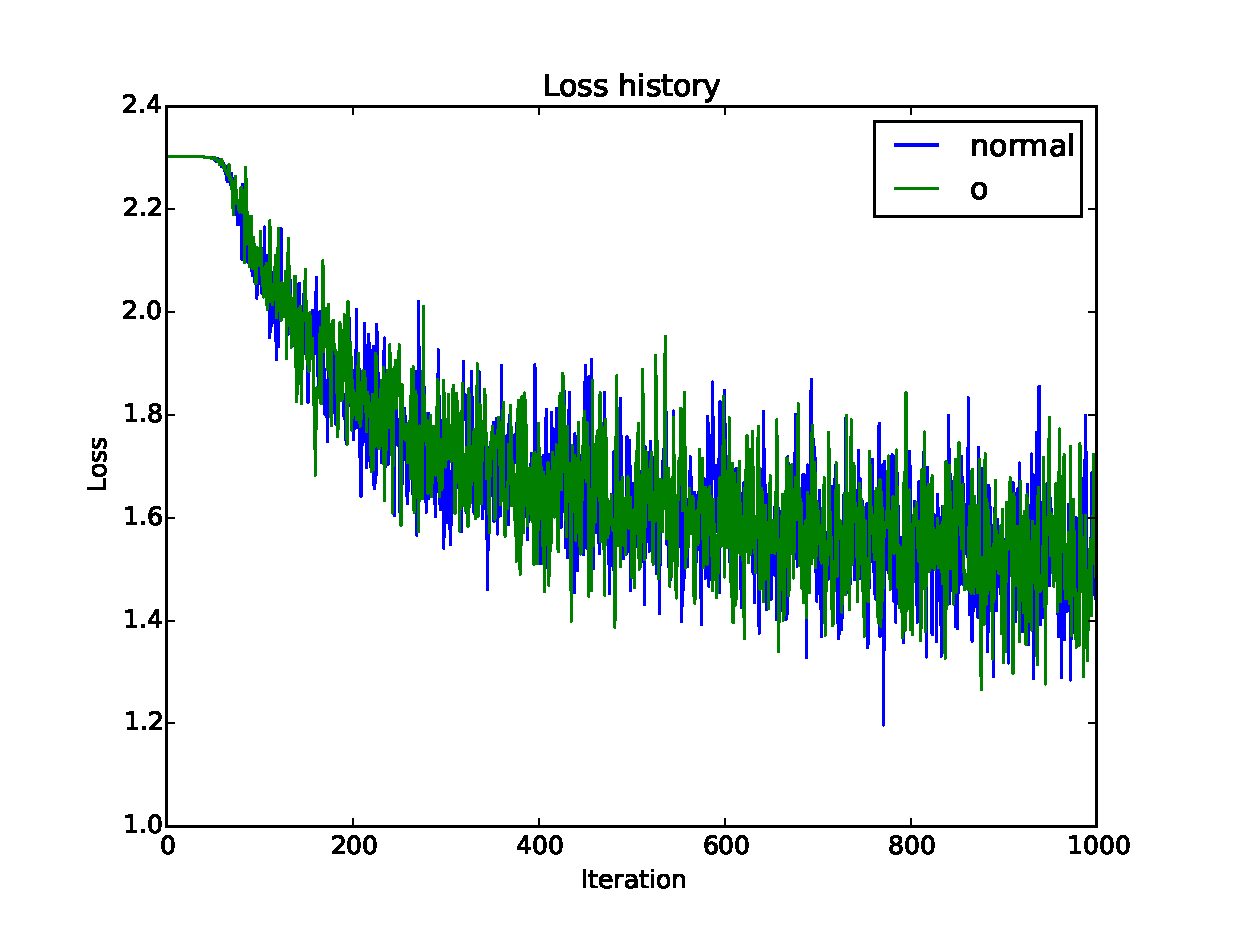
\includegraphics[width=\columnwidth]{loss}
 			% Create a subtitle for the figure.
 			% Define the label of the figure. It's good to use 'fig:title', so you know that the label belongs to a figure.
 			\label{fig:tf_plot}
 		\end{center}
 	\end{figure}
 
 
	
\subsection{Activation functions}
  I've tried 2 activation functions except ReLU: \emph{leaky ReLU} and \emph{tanh}. 
  
  Implementation of leaky RelU needs to change a few lines of forward pass and backpropagation. $\alpha$ is set emperically.
\begin{lstlisting}
#forward pass
a2=np.maximum(inp,.01*inp)
#backpropagation
dF=np.ones(np.shape(a2))
dF[a2<0.0]=0.01
\end{lstlisting}
  As is mentioned in research, leaky ReLU may lead to overfitting sometimes. In my test, with the same other hyperparameters, 
  training accuracy of leaky ReLU improved by 4\%, however, validation accuracy seems not improved.
  
  As for \emph\emph{tanh}, with the same other hyperparameters, training time becomes longer, and validation accuracy dropped 2\%.
  
\subsection{Preprocessing}
  I employ PCAwhitening and K-means to do data preprocessing. It turns out that these two processes hugely improve test accuracy.
  Without special tuning, test accuracy could easily reach 65\%. By intuition, PCAwhithening reduce effects of bright and contract,
  and K-means put images into different classes before we truely begin training.
  
  I use np.lingalg to implement PCAwhitening as follow:
\begin{lstlisting}
[D,V]=np.linalg.eig(
  np.cov(img,rowvar=0))
P = V.dot(
  np.diag(np.sqrt(1/(D + 0.1))))
    .dot(V.T)
img = img.dot(P)
\end{lstlisting}
  Intuitively, Kmeans clusters different images into different clusters, which is much easier for our neural net to handle. 
  I select 1600 centroids emperically from previous work. Also I encountered \emph{MemoryError} 
  when implementing Kmeans, because our data can not be clustered at once. So I changed the 
  processing way a little bit:
\begin{lstlisting}
for each iterations:
  for each batch in data:
    cluster batch
    cumulate result
  renew centroids
\end{lstlisting}
  Finally, with these PCAwhitening and K-means, my best test accuracy successfully reaches \textbf{74\%}. 
  The following two graphs shows loss history and training, validation accuracy of the selected best hyperparameters.
  More details of hyperparameters is shown in the next section.
  \begin{center}
 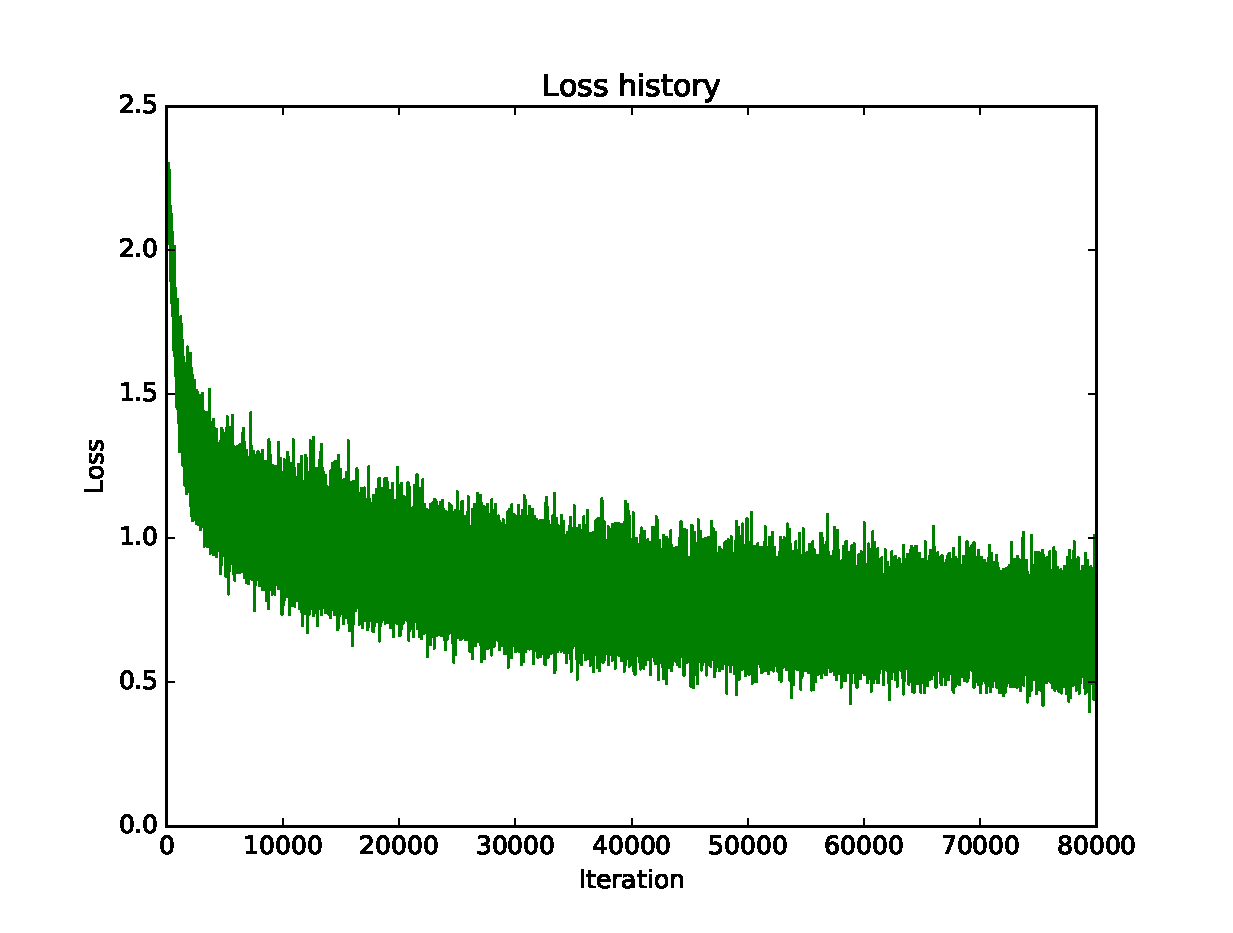
\includegraphics[width=\columnwidth]{./kmeans_his.eps}
 % kmeans_his.eps: 0x0 pixel, 300dpi, 0.00x0.00 cm, bb=18 180 594 612
  \end{center}
  \begin{center}
 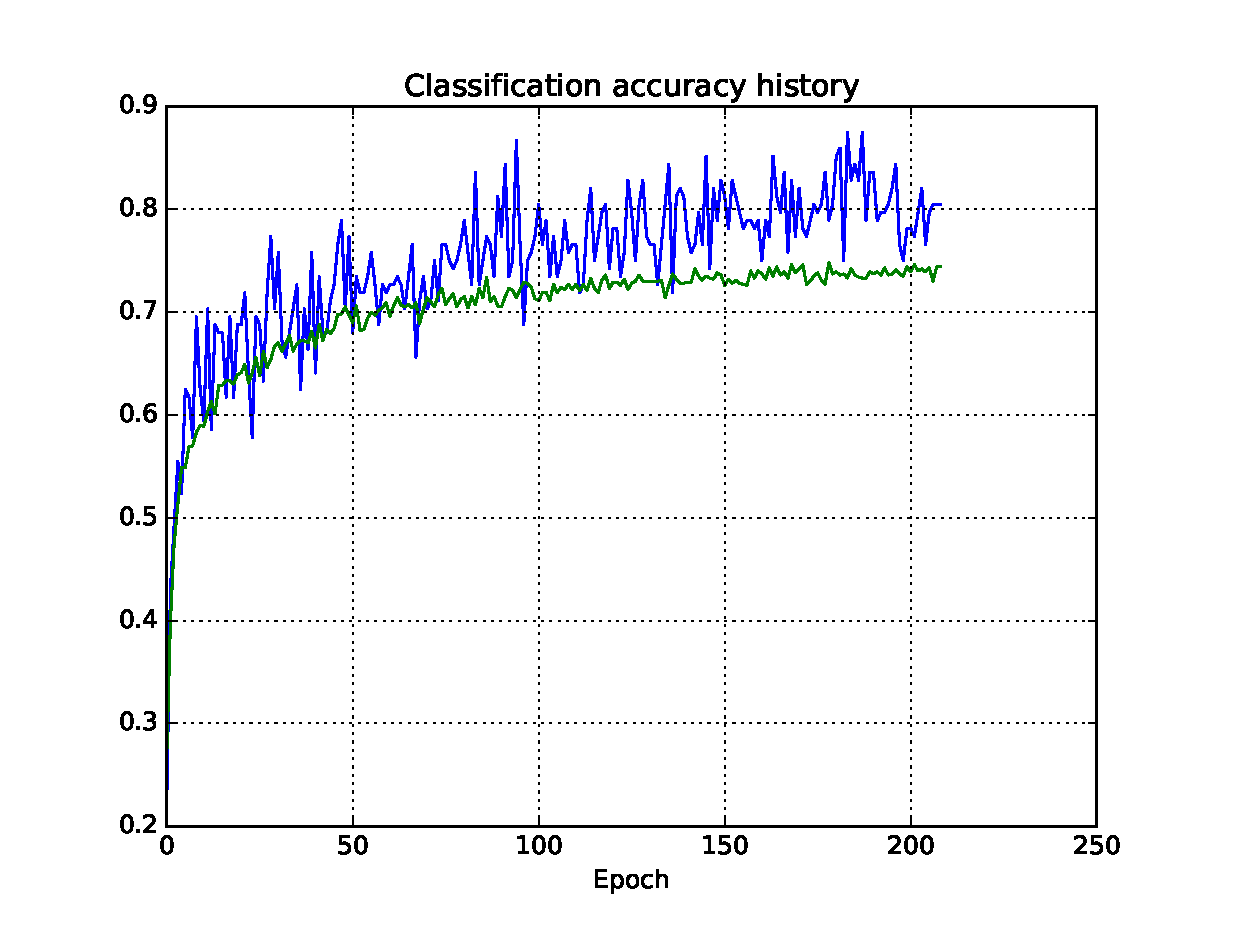
\includegraphics[width=\columnwidth]{./kmeans_acc.eps}
 % kmeans_his.eps: 0x0 pixel, 300dpi, 0.00x0.00 cm, bb=18 180 594 612
  \end{center}
  Due to our time limitation, I choose to use 200 hidden nodes. I guess it will work better with more hidden nodes,
  and longer training time. 
  
\section{Results}
  As mentioned in II Model Building, I employed a grid search to find best hyperparameters. 
  In order to get better result, I tuned number of iterations, 
  finally fix it to 12000, with a batch size of 100. It increases the Validation accuracy 5\%. 
  
  The following table shows my three methods accuracy:
    \begin{table}[!hbt]
    	\centering
    	\caption{Differences between update methods}
    	\label{Differences between update methods}
    	\begin{tabular}{lllll}
				& Naive & Dropout & Preprocessed & \\
	  hidden nodes    & 350   & 500        & 200 & \\
	  learning rate & $1\times10^{-3}$   & $1\times10^{-4}$       & $5\times10^{-4}$ &  \\
	  learning rate Decay & .95   & .95       & .99 &  \\
	  regularization & L2,0.05  & Dropout,.5       & Dropout,.3 &  \\
	  Activation  & ReLU  & Leaky ReLU       & ReLU &  \\
	  Update method  & SGD  & Momentum,0.9       & Momentum,0.95   &  \\
	  Iterations & $1\times10^{4}$  & $1\times10^{4}$       & $7\times10^{4}$ &  \\    		
	  Batch size & 100  & 100       & 128 &  \\    		
	  Time(min)  & 15  & 80       & 110 &     		\\
	  Train accuracy  & 60\%  & .458       & .80 & \\
			Validation  & 55\%  & .458       & .75 &     	\\	
    		Test  & 51.6\%  & .55       & .74 &     		
    		
    	\end{tabular}
    \end{table}
    

% You can cite a book or paper by using \cite{reference}.
% The references will be defined at the end of this .tex file in the bibliography
% References should be cited as numbers, and should be ordered by their appearance (example: ``... as shown in \cite{HOP96}, ...'').
% Only references that are actually cited can be listed in the references section.
% The references' format should be evident from the examples in this text.
% 
% References should be of academic character and should be published and accessible.
% Your advisor can answer your questions regarding literature research.
% You must cite all used sources.
% Examples of good references include text books and scientific journals or conference proceedings.
% If possible, citing internet pages should be avoided. In particular, Wikipedia is \emph{not} an appropriate reference in academic reports.
% Avoiding references in languages other than English is recommended.






\section{Challenges}
	I encountered many challenges through this machine problem
	
	When I'm doing gradient check. I spent great amount of time finding bugs in my code,
	but still not able to figure out what's wrong with my code. 
	Then, instead of directly comparing gradient errors, 
	I cut gradient check procedure into pieces. 
	Check derivatives sequentially:
	$\frac{\partial H}{\partial a^{(3)}}$,$\delta^{(3)}$,
	$\frac{\partial H}{\partial w^{(2)}}$,$\frac{\partial H}{\partial b^{(2)}}$,$\delta^{(2)}...$
	
	Tuning hyperparameters is really time consuming, I run my program on both on my laptop and CSIL lab. And create 
	multi threads to speed up. I save training infomations like hyperparameters and accuracy to \emph{CSV} files. View
	them when the program finish. It saves me a lot of time and avoids hand tuning.
	
  Some parts of my code encountered \emph{MemoryError}, 
  because operation like matrix multiplications. I tried iteration way and 
  batch way of matrix multiplications. Both solve \emph{MemoryError}, but batch way turns out to be much faster.
	
\section{Possible Improvements}
  There are some other update methods(Adam, Adagrad, etc) I haven't tried. 
  Maybe they are better than Momentum and RMSprop.

  More complexed activation function like PReLU, maybe work better than ReLU and Leaky ReLU.
  
  L1 regularization in some situation, maybe better than L2.
  
  As for preprocessing, applying kernel trick may improve results.
  
  With longer training time, it is possible to reach higher accuracy.
  
% Now we need a bibliography:
% \begin{thebibliography}{5}
% 
% 	%Each item starts with a \bibitem{reference} command and the details thereafter.
% 	\bibitem{HOP96} % Transaction paper
% 	J.~Hagenauer, E.~Offer, and L.~Papke. Iterative decoding of binary block
% 	and convolutional codes. {\em IEEE Trans. Inform. Theory},
% 	vol.~42, no.~2, pp.~429�C-445, Mar. 1996.
% 
% 	\bibitem{MJH06} % Conference paper
% 	T.~Mayer, H.~Jenkac, and J.~Hagenauer. Turbo base-station cooperation for intercell interference cancellation. {\em IEEE Int. Conf. Commun. (ICC)}, Istanbul, Turkey, pp.~356--361, June 2006.
% 
% 	\bibitem{Proakis} % Book
% 	J.~G.~Proakis. {\em Digital Communications}. McGraw-Hill Book Co.,
% 	New York, USA, 3rd edition, 1995.
% 
% 	\bibitem{talk} % Web document
% 	F.~R.~Kschischang. Giving a talk: Guidelines for the Preparation and Presentation of Technical Seminars.
% 	\url{http://www.comm.toronto.edu/frank/guide/guide.pdf}.
% 
% 	\bibitem{5}
% 	IEEE Transactions \LaTeX and Microsoft Word Style Files.
% 	\url{http://www.ieee.org/web/publications/authors/transjnl/index.html}
% 
% \end{thebibliography}

% Your document ends here!
\end{document}